\chapter{Lecture 14: Geometric, Poisson, and negative binomial distribution}
\section{Geometric distribution} \label{Geometric distribution}
Take a moment to review the binomial distribution in section \ref{binom pmf}. Recall that the number of trials $n$ is fixed, while the number of successes is counted by $X$ (the random variable). \\

\noindent Suppose we have the same situation (identical and independent Bernoulli trials, with success probability $p$), except that we make $X$ count the \textit{number of trials} rather than the number of successes. We fix the number of successes at $1$; so, we are counting the number of trials up to and including the first success. \\

\noindent The possible values of $X$ are $X \in \set{1,2,3,\ldots}$. We have one parameter, $p$ (probability of success on each trial). If $X = k$, then this means we had failures on the first $k - 1$ trials and success on the $k^{\text{th}}$ trial. \\

\noindent Since the probability of success is $p$, the probability of failure on each trial must be $1-p$. We want to find the probability of ``failure on trial 1 \textit{and} failure on trial 2 \textit{and} \ldots \textit{and} success on trial $k$. The probabilities associated with each trial can be multiplied together to find the probability of the intersection of the trials, since the trials are independent from eachother (remember, intersect translates roughly to ``$\textit{and}$''). Hence, we define a rule, $p(k)$, for the \textbf{the probability mass function of the geometric distribution with success parameter $\boldsymbol{p}$}, as follows

  	\bigskip
	
	\hfil\fbox{
	\begin{minipage}{0.7\columnwidth}{
	
	%\vskip 0.05cm
	\begin{center}
	$\displaystyle{P(X = k) = p(k) = (1-p)^{k-1}p \;\;\; \text{where $k \in \set{1,2,3,\ldots}$}}$
	\end{center}
	}
	\end{minipage}}
	\bigskip
	\bigskip

\noindent Which multiplies $(1-p)$ together for $k-1$ times (the number of failures), then multiplies all this by $p$ once (the number of successes). We can write \textbf{Geom($\boldsymbol{p}$)} for short. \\

\noindent Below is a plot of the pmf for Geom($0.5$), for $k \in \set{1,2,3,4,5}$.
\begin{center}
\begin{tikzpicture}[xscale = 1, yscale = 10]
\draw [->,gray] (0,-0.01) -- (0,0.6) node [above left] {$p(k)$};
\draw [->,gray] (-0.1,0) -- (6,0) node [below right] {$k$};
\foreach \x in {1,2,3,4,5}{
\draw (\x,0) node {$|$} node [below = 2mm] {$\x$};
}
\foreach \y in {0.1,0.2,0.3,0.4,0.5}{
\draw (0.1,\y) -- (-0.1,\y) node [left] {$\y$};
}
\draw [fill = black] (1,0.5) ellipse (0.1cm and 0.01cm);
\draw [fill = black] (2,0.25) ellipse (0.1cm and 0.01cm);
\draw [fill = black] (3,0.125) ellipse (0.1cm and 0.01cm);
\draw [fill = black] (4,0.0625) ellipse (0.1cm and 0.01cm);
\draw [fill = black] (5,0.03125) ellipse (0.1cm and 0.01cm);
\end{tikzpicture}
\end{center}

\subsection{Example} \label{mode1(notreally)}
What is the \textit{mode} of the geometric distribution? Note that ``mode'' is the event which has the highest associated probability. Hint: Consider $\frac{P(X=k+1)}{P(X=k)}$ \\

\noindent \textit{Solution:} \\
Looking at the pmf for Geom(0.5) in the previous graph, we can see that $P(X = k)$ is highest when $k = 1$, and decreases for increasing $k$. To prove that $X = 1$ is the mode in general would require us to prove that the geometric distribution is, in general, always decreasing. We can do this by looking at the ratio of each term to the next, i.e.,
\[
\frac{P(X=k+1)}{P(X=k)} = \frac{p(k+1)}{p(k)} = \frac{p(1-p)^k}{p(1-p)^{k-1}} = (1-p) \tag{index laws}
\] 
So the ratio is $1-p$. Now, assuming we have non-zero probability of success, we know that $0 < p \leq 1$. Multiplying through this inequality by $-1$ gives $0 > -p \geq -1$. Adding $1$ to all sides gives $1 >1 - p \geq 0$. So $1-p$ (the ratio of each output to the next) is a number whose magnitude is less than $1$; this means that the outputs are always getting smaller (decreasing). Hence we conclude that the first output, $P(k = 1)$, must be the greatest.


\subsection{Example}
30\% of applicants for a drug trial actually have the condition of interest. If applicants are interviewed for the trial sequentially and randomly from a pool, what is the probabillity of first finding one who has the condition on the fifth interview?

\noindent \textit{Solution:} \\
Let $X$ be the discrete random variable counting the number of trials up to and including the first success. This is a case of identical, independent trials that result in success or failure. The probability of success is $p = 0.3$. So $X \sim $ Geom($0.3$). Hence
\[
P(X = 5) = (1-0.3)^{4}0.3 = 0.7^40.3 = 0.0720
\]

\subsection{Checking validity of Geom($\boldsymbol{p}$)}
With each new distribution that we introduce, it is customary for us to check that its pmf satisfies the probability measure axioms. Just like before, Axiom 3 is not something we need to check (see section \ref{validity of bin}). Checking axiom 2 is an easy exercise left to the reader (axiom 2 says we require $p(k) \geq 0$ for all possible $k$). We need only check axiom 1 here (that $P(\Omega) = 1$, i.e., that the probabilities sum to 1). \\

\noindent Recall the infinite geometric series (from section \ref{geometric series}); it is defined to be the sum of a sequence whose terms differ only by a common ratio, $a$, and $c$ is some constant:
\[
\sum_{k=0}^\infty ca^k = c + ca + ca^2 + ca^3 + \ldots = \frac{c}{1-a} \tag{$\bigstar$}
\]
The outputs of the pmf of the geometric distribution also have a common ratio (the common ratio is $a = 1-p$, and the constant is $c = p$). The sum, over all possible $k$, of the outputs is
\begin{align*}
\sum_{k=1}^\infty P(X = k) = \sum_{k=1}^\infty p(1-p)^{k-1} & = p + p(1-p) + p(1-p)^2 + p(1-p)^3 + \ldots \\
	& = \frac{p}{1-(1-p)} \tag{by the formula ($\bigstar$) above} \\
	& = \frac{p}{p} = 1.
\end{align*}
So axiom 1 is satisfied.

\subsection{Cumulative distribution function for Geom($\boldsymbol{p}$)} \label{geom cdf} \label{finite geometric series}
To find the cdf, we need to use the formula for the sum of the \textbf{finite geometric series}, which we have not met yet (the proof is given in appendix \ref{appendixD}). The formula is
\[
\sum_{k=0}^n ca^k = c\frac{1-a^{n+1}}{1-a}. \tag{$\spadesuit$}
\]
Remember, a cdf is defined to be the function, $F(k)$, whose output is $P(X \leq k)$. Now, in section \ref{validity of bin} (under the heading, ``axiom 3'') we spoke about the reason why $P(X \leq k) = \sum_{i = 1}^k P(X = i)$ (we actually spoke about the general case, but this is the case where $k \geq 1$). Incorporating this fact, we have
\begin{align*}
F(k) = P(X \leq k) & = \sum_{i = 1}^k P(X = i) \tag{see section \ref{validity of bin} (axiom 3) for why this is true} \\
	& = \sum_{i = 1}^k p(1-p)^{i-1} \\
	& = p + p(1-p) + p(1-p)^2 + \ldots + p(1-p)^{k-1} \\
	& = \sum_{i = 0}^{k-1} p(1-p)^i \\
	& = p\frac{1-(1-p)^k}{1-(1-p)} \tag{by ($\spadesuit$); with $c = p, a = 1-p,$ and $n = k - 1$} \\
	& = p\frac{1-(1-p)^k}{p} \\
	& = 1-(1-p)^k.
\end{align*}
Which is a nice neat rule for the cdf of the geometric distribution.

\section{Poisson distribution}
The Poisson distribution is another distribution that can be related to Bin($n,p$). For the binomial distribution, we conduct $n$ trials, and each trial has some probability, $p$, of success. For example, we might be driving past the post box once every day, and we might be wondering how many times we are likely to see the post officer collect the mail over the course of one week (7 distinct trials). Success is when we spot the post officer, and failure is when we do not. The Poisson distribution comes in handy when we can no longer distinguish one trial from another. For example, we might just be driving around, on one long drive, and wonder how many post officers we are likely to spot driving past us. We are still dealing with success or failure (spotting or not spotting a post officer) but there is no separation between trials - we are on one long drive and could spot a post officer at any time. \\

\noindent Rare events which occur in a continuum (e.g., space, time, or volume) are modelled by the Poisson distribution. The only parameter for this distribution is $\lambda$, the average number of occurrences of the event per unit of the continuum. \smallskip \label{lambda poisson}

\begin{center}
\begin{tabular}{|c|c|c|} \hline
 \textbf{Event}	& \textbf{Continuum} & \textbf{Example $\boldsymbol{\lambda}$} \\ \hline
Traffic accidents & Time 	      & $\frac{\text{avg no. traffic accidents}}{\text{1 hour}}$ \\ \hline
Flaws in cloth 	 &  Area	     & $\frac{\text{avg no. flaws}}{\text{1 square meter}}$ \\ \hline
Starfish 		 & Length (of reef) & $\frac{\text{avg no. starfish}}{\text{1 kilometer}}$ \\ \hline
Emails 		 & Time 	     & $\frac{\text{avg no. emails}}{\text{1 day}}$ \\ \hline
Reactions to vaccine & volume (of patients) & $\frac{\text{avg no. reactions}}{\text{10 patients}}$ \\ \hline
\end{tabular}
\end{center}
We now give the \textbf{pmf for the Poisson distribution}, without a derivation. The probability of $k$ occurrences in one unit of continuum is \label{poi(lambda)}

  	\bigskip
	
	\hfil\fbox{
	\begin{minipage}{0.3\columnwidth}{
	
	%\vskip 0.05cm
	\begin{center}
	$\displaystyle{P(X = k) = \frac{\lambda^k}{k!}\e^{-\lambda}}$
	\end{center}
	}
	\end{minipage}}
	\bigskip
	\bigskip

\noindent We can write Poi($\lambda$) for short. Note that we always have $\lambda \geq 0$. \\

\noindent The binomial distribution, Bin($n,p$), approaches the poisson distribution when $n$ is very large, and $p$ is very small. The parameter $\lambda$ is then given by $\lambda = np$ (which should itself be neither too large nor too small). For example, if we have $n \geq 100, p \leq 0.01,$ and $np \leq 20$, then Bin($n,p$) will very closely resemble Poi($\lambda$). \\

\noindent It can be shown that if $n \rightarrow \infty$, $p \rightarrow 0$, and $\lambda = np$ remains constant, then, in this limit, the two distributions become equal. The proof is given in appendix \ref{appendixE}. To understand this intuitively, you can image that 1 unit of continuum (e.g., 1 minute of time) is broken down into $n$ subintervals (e.g., we might break a minute down into seconds). The average number of occurrences per unit is $\lambda$, so the average number of occurrences when we break the unit into $n$ subintervals is $\frac{\lambda}{n}.$ If we make $n$ so large (i.e., make the subintervals so infinitesimally small) that only one occurrence could happen in each subinterval, then we can view each subinterval as a single trial from the binomial ditribution. Hence the probability of an occurrence for each trial is $p = \frac{\lambda}{n}$; which we can rearrange to $\lambda = np.$


%
%\subsubsection{Proof}
%Let $X \sim $ Bin($n,p$). Since $\lambda = np$, we rearrange to get $p = \frac{\lambda}{n}$. Now,
%\begin{align*}
%P(X = k) & = \binom{n}{k}p^k(1-p)^{n-k} \tag{this is the pmf of Bin($n,p$)} \\
%	& = \frac{n!}{k!(n-k)!}p^k(1-p)^{n-k} \tag{expanding the binomial coefficient} \\
%	& = \frac{n!}{\boldsymbol{k!}(n-k)!}\brac{\frac{\boldsymbol{\lambda}}{n}}^{\boldsymbol{k}} \brac{1-\frac{\lambda}{n}}^{n-k} \tag{since $p = \frac{\lambda}{n}$} \\
%	& = \boldsymbol{\frac{\lambda^k}{k!}} \frac{n!}{(n-k)!n^k} \brac{1-\frac{\lambda}{n}}^{n-k} \tag{the $k!$ and $\lambda^k$ (in bold) were moved} \\
%	& =  \boldsymbol{\frac{\lambda^k}{k!}} \frac{n!}{(n-k)!n^k}\brac{1-\frac{\lambda}{n}}^{n}\brac{1-\frac{\lambda}{n}}^{-k} \tag{index laws}
%\end{align*}
%So far we have just expressed the pmf for Bin($n,p$) in a different way. Now we need to take the limit as $n \rightarrow \infty$ of this expression. Note that $\frac{\lambda^k}{k!}$ is a constant, so we can pull it outside the limit (since limits are linear). Hence
%\begin{align*}
%\lim_{n \rightarrow \infty}\brac{P(X = k)} & = \frac{\lambda^k}{k!}\lim_{n \rightarrow \infty}\brac{\frac{n!}{(n-k)!n^k}\brac{1-\frac{\lambda}{n}}^{n}\brac{1-\frac{\lambda}{n}}^{-k}}
%\end{align*}
%The right hand side is a product of three sequences; a useful result about limits tells us that the limit of a product is equal to the product of the limits (see section \ref{limitfacts}). \\
%
%Now, 

\subsection{Example}
Giant sea monsters (worse than sharks), on the planet Seabad, follow a Poisson distribution with $\lambda = 15$ sea monsters per meter squared. The onboard computer is trying to decide on a recommendation regarding an emergency landing on this planet. What is the probability of finding no sea monsters within a circle of area 10 square meters (around your landing vessel)? \\

\noindent \textit{Solution:} \\
Let $X$ be the discrete random variable that counts the number of sea monsters within a circle of area 10 square meters. Then $X \sim $ Poi($\alpha$) for some $\alpha$. Since there are an average of $\lambda = 15$ sea monsters per meter squared, it follows that there are an average of $10\times15 = 150$ sea monsters per 10 meters squared. Hence $\alpha = 150.$ So using the pmf of Poi($150$) we get, 
\[
P(X = 0) = \frac{150^0}{0!}\e^{-150} \approx 0.
\]
Conclusion: Do not land on planet Seabad.

\subsection{Checking validity of Poi($\boldsymbol{\lambda}$)} \label{check poi(lambda)}
As usual, we will only check that the pmf satisfies probability measure axiom 1 (axiom 2 is left to the reader). As usual, for random variables, checking axiom 1 is equivalent to checking that the probabilities sum to 1. We have
\begin{align*}
\sum_{k=0}^\infty P(X = k) & = \sum_{k=0}^\infty \frac{\lambda^k}{k!}\e^{-\lambda} \tag{using pmf of Poi($\lambda$)} \\
	& = \e^{-\lambda}\sum_{k=0}^\infty \frac{\lambda^k}{k!} \tag{since $\e^{-\lambda}$ is constant and sums are linear} \\
	& = \e^{-\lambda} \times \e^{\lambda} \tag{using power series definition of $\e^x$ (see section \ref{power series})} \\
		& = \e^0 = 1. \tag{index laws}
\end{align*}
So axiom 1 is satisfied.

\subsubsection{Visualising the Poisson distribution}
Below are some graphs of the Poisson distribution for different $\lambda$
\begin{center}
	\begin{tikzpicture}[xscale = 2, yscale = 10]
	\draw [->,gray] (0,-0.03) -- (0,0.65) node [above left] {$p(k)$};
	\draw [->,gray] (-0.1,0) -- (3.25,0) node [below right] {$k$};
	\foreach \x in {1,2,3}{
	\draw (\x,0) node {\tiny{$|$}} node [below = 2mm] {$\x$};
	}
	\foreach \y in {0.1,0.2,0.3,0.4,0.5,0.6}{
	\draw (0.05,\y) -- (-0.05,\y) node [left] {$\y$};
	}
	\draw [fill = black] (0,0.607) ellipse (0.05cm and 0.01cm);
	\draw [fill = black] (1,0.303) ellipse (0.05cm and 0.01cm);
	\draw [fill = black] (2,0.0758) ellipse (0.05cm and 0.01cm);
	\draw [fill = black] (3,0.01263) ellipse (0.05cm and 0.01cm);
	\draw (2,0.5) node {Poi($\frac{1}{2}$)};
	\end{tikzpicture}
\end{center}
\begin{center}
	\begin{tikzpicture}[xscale = 1.4, yscale = 14]
	\draw [->,gray] (0,-0.03) -- (0,0.45) node [above left] {$p(k)$};
	\draw [->,gray] (-0.1,0) -- (4.5,0) node [below right] {$k$};
	\foreach \x in {1,2,3,4}{
	\draw (\x,0) node {\tiny{$|$}} node [below = 2mm] {$\x$};
	}
	\foreach \y in {0.1,0.2,0.3,0.4}{
	\draw (0.05,\y) -- (-0.05,\y) node [left] {$\y$};
	}
	\draw [fill = black] (0,0.3679) ellipse (0.07cm and 0.007cm);
	\draw [fill = black] (1,0.3679) ellipse (0.07cm and 0.007cm);
	\draw [fill = black] (2,0.1839) ellipse (0.07cm and 0.007cm);
	\draw [fill = black] (3,0.0613) ellipse (0.07cm and 0.007cm);
	\draw [fill = black] (4,0.0153) ellipse (0.07cm and 0.007cm);
	\draw (3,0.3) node {Poi($1$)};
	\end{tikzpicture}
\end{center}
\begin{center}
	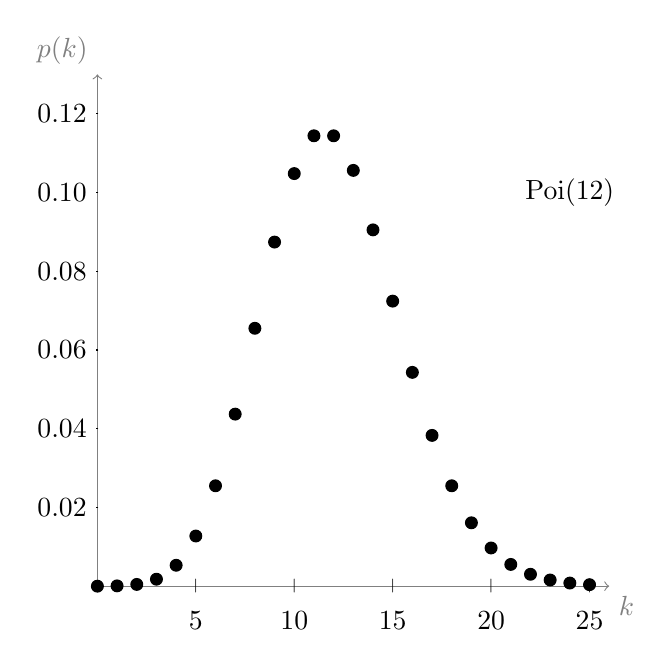
\begin{tikzpicture}[xscale = 0.25, yscale = 50]
	\draw [->,gray] (0,-0.0005) -- (0,0.13) node [above left] {$p(k)$};
	\draw [->,gray] (-0.1,0) -- (26,0) node [below right] {$k$};
	\foreach \x in {5,10,15,20,25}{
	\draw (\x,0) node {\tiny{$|$}} node [below = 2mm] {$\x$};
	}
	\foreach \y in {0.02,0.04,0.06,0.08,0.10,0.12}{
	\draw (0.05,\y) -- (-0.05,\y) node [left] {$\y$};
	}
	\draw [fill = black] (0,0.00000614) ellipse (0.3cm and 0.0015cm);
	\draw [fill = black] (1,0.00007373) ellipse (0.3cm and 0.0015cm);
	\draw [fill = black] (2,0.000442) ellipse (0.3cm and 0.0015cm);
	\draw [fill = black] (3,0.0017695) ellipse (0.3cm and 0.0015cm);
	\draw [fill = black] (4,0.0053086) ellipse (0.3cm and 0.0015cm);
	\draw [fill = black] (5,0.01274) ellipse (0.3cm and 0.0015cm);
	\draw [fill = black] (6,0.0255) ellipse (0.3cm and 0.0015cm);
	\draw [fill = black] (7,0.0437) ellipse (0.3cm and 0.0015cm);
	\draw [fill = black] (8,0.0655) ellipse (0.3cm and 0.0015cm);
	\draw [fill = black] (9,0.0874) ellipse (0.3cm and 0.0015cm);
	\draw [fill = black] (10,0.1048) ellipse (0.3cm and 0.0015cm);
	\draw [fill = black] (11,0.1144) ellipse (0.3cm and 0.0015cm);
	\draw [fill = black] (12,0.1144) ellipse (0.3cm and 0.0015cm);
	\draw [fill = black] (13,0.1056) ellipse (0.3cm and 0.0015cm);
	\draw [fill = black] (14,0.0905) ellipse (0.3cm and 0.0015cm);
	\draw [fill = black] (15,0.0724) ellipse (0.3cm and 0.0015cm);
	\draw [fill = black] (16,0.0543) ellipse (0.3cm and 0.0015cm);
	\draw [fill = black] (17,0.0383) ellipse (0.3cm and 0.0015cm);
	\draw [fill = black] (18,0.0255) ellipse (0.3cm and 0.0015cm);
	\draw [fill = black] (19,0.0161) ellipse (0.3cm and 0.0015cm);
	\draw [fill = black] (20,0.0097) ellipse (0.3cm and 0.0015cm);
	\draw [fill = black] (21,0.00553) ellipse (0.3cm and 0.0015cm);
	\draw [fill = black] (22,0.00302) ellipse (0.3cm and 0.0015cm);
	\draw [fill = black] (23,0.00157) ellipse (0.3cm and 0.0015cm);
	\draw [fill = black] (24,0.000787) ellipse (0.3cm and 0.0015cm);
	\draw [fill = black] (25,0.000378) ellipse (0.3cm and 0.0015cm);
	\draw (24,0.10) node {Poi($12$)};
	\end{tikzpicture}
\end{center}
We loosly defined the term ``mode'' in section \ref{mode1(notreally)}, we will define it in more detail in section \ref{mode definition}. We can see from the graphs that for $\lambda = \frac{1}{2}$ the mode  is at $k = 0$. We can also see that for $\lambda = 1$ the mode can be $0$ or $1$, and for $\lambda = 12$ the mode can be $11$ or $12$. Why is the mode moving to the right as $\lambda$ increases? We should be able to find a formula for the mode, which is somehow dependent on lambda. \\

\noindent A good place to start is by looking at the ratio of each term to the next. We have
\begin{align*}
\frac{P(X = k+1)}{P(X=k)} & = \frac{\lambda^{k+1}}{(k+1)!}\e^{-\lambda} \times \frac{k!}{\lambda^k}\e^{\lambda}  \\
	& = \frac{\lambda^{k+1}}{\lambda^k}\frac{k!}{(k+1)!}e^0 \\
	& = \frac{\lambda}{k+1}.
\end{align*}
So, when $\frac{\lambda}{k+1} > 1$, the probability will be increasing, and when $\frac{\lambda}{k+1} < 1$ the probability will be decreasing. \\

\noindent Let's have a look at what happens when $\lambda > 1$. Since $k+1$ starts off small (with $k = 0$), it follows that $k+1 < \lambda$ (meaning that $\frac{\lambda}{k+1} > 1$) to start off with; then, as $k$ grows in size, it gets closer to the size of $\lambda$, and we eventually get near $k+1 = \lambda$ (the mode will be around here), $k$ will then keep increasing until $k + 1 > \lambda$ (meaning that $\frac{\lambda}{k+1} < 1$), and thus the probability will continue decreasing as $k$ keeps increasing. In conclusion, there will always be a mode around the point where $k+1 = \lambda$.  \\

\noindent Now let's have a look at what happens when $\lambda \leq 1$. Again $k+1$ starts off small (with $k = 0$), but since $k = 0$ we have $k+1 = 0 + 1 \geq \lambda$ to start off with (since $\lambda \leq 1$). Hence $\frac{\lambda}{k+1} \leq 1$ already, and as $k$ keeps increasing this ratio will keep getting smaller. In conclusion, there will always be a mode around $k = 0$ when $\lambda < 1$.  

\section{Negative binomial distribution} \label{negbin(r,p)}
For Geom($p$) we had identical and independent Bernoulli trials, with success probability $p$; the random variable counts the number of trials up to and including the \textit{first} success. \\

\noindent Suppose we have the same situation, except that we wish to conduct trials until seeing $r$ successes. So the random variable, say $X$, counts the number of trials up to and including the $r^{\text{th}}$ success. \\

\noindent Suppose we get $X = k$.  The outcomes of the trials (i.e., the events) are independent, so the probability of their intersect is the product of their probabilities. There are multiple ways that this could happen, but the probability associated with any particular arrangement is
\[
p^r(1-p)^{k-r}
\]
\noindent The final trial is always a success (so this can happen in only 1 way), and among the other $k-1$ trials, we had $r - 1$ successes. The number of (unordered) ways of choosing $r-1$ successes from $k-1$ trials is $\binom{k-1}{r-1}$. Hence

  	\bigskip
	
	\hfil\fbox{
	\begin{minipage}{0.4\columnwidth}{
	
	%\vskip 0.05cm
	\begin{center}
	$\displaystyle{P(X = k) = \binom{k-1}{r-1}p^r(1-p)^{k-r}.}$
	\end{center}
	}
	\end{minipage}}
	\bigskip
	\bigskip

\noindent This is the pmf of the \textbf{negative binomial ditribution with parameters $\boldsymbol{r}$ and $\boldsymbol{p}$.} The abbreviation is NegBin($r,p$). \\ 

\noindent \textbf{Important!!} Always remember that the trials \textit{must be independent and identical Bernoulli trials} for us to use any one of Bin($n,p$), Geom($p$), or NegBin($r,p$). If we are, for example, selecting items without replacement from a (not very large) pool of items, then the trials will not be identical, since the pool of items grows smaller with each selection; in this case consider using the hypergeometric distribution instead (which applies when the trials are not identical in nature). It is common for people to confuse some situations that deserve the hypergeometric distribution for ones that deserve NegBin($r,p$). \\

\noindent The geometric distribution is in fact a special case of the negative binomial distribution. We can recover the pmf of Geom($p$) from NegBin($r,p$) by letting $r = 1$; we get,
\[
P(X = k) = \binom{k-1}{1-1}p^1(1-p)^{k-1} = \binom{k-1}{0}p(1-p)^{k-1} = p(1-p)^{k-1}.
\]
Which is the pmf of Geom($p$), as required. So Geom($p$) = NegBin($1,p$). \\

\noindent Also be aware that that there exists one other variation (which we do not cover here), of the negative binomial distribution, in which $X$ counts the number of failures after $r$ successes, rather than the number of trials. This variation has a different pmf. However, if there are $q$ failures, then there are $q+r$ trials, so to get from the graph of one variation to the other is just a matter of shifting the values along the $x$-axis by the value $q$. \\ 

\noindent Below are some plots of the pmf for NegBin($r,p$). Note that the pmf is undefined where $k < r$. So, for example, for NegBin($10,\frac{1}{2}$) we plot only for $k \geq 10$.
\begin{center}
	\begin{tikzpicture}[xscale = 0.3, yscale = 60]
	\draw [-latex,gray] (10,-0.003) -- (10,0.1) node [above left] {$p(k)$};
	\draw [-latex,gray] (10-0.1,0) -- (32,0) node [below right] {$k$};
	\foreach \x in {10,15,20,25,30}{
	\draw (\x,0) node {\tiny{$|$}} node [below = 2mm] {$\x$};
	}
	\foreach \y in {0.01,0.03,0.05,0.07,0.09}{
	\draw (10+0.2,\y) -- (10-0.2,\y) node [left] {$\y$};
	}
	\draw [fill = black] (10,0.00098) ellipse (0.2cm and 0.001cm);
	\draw [fill = black] (11,0.00488) ellipse (0.2cm and 0.001cm);
	\draw [fill = black] (12,0.0134) ellipse (0.2cm and 0.001cm);
	\draw [fill = black] (13,0.0269) ellipse (0.2cm and 0.001cm);
	\draw [fill = black] (14,0.04364) ellipse (0.2cm and 0.001cm);
	\draw [fill = black] (15,0.061096) ellipse (0.2cm and 0.001cm);
	\draw [fill = black] (16,0.07637) ellipse (0.2cm and 0.001cm);
	\draw [fill = black] (17,0.08728) ellipse (0.2cm and 0.001cm);
        	\draw [fill = black] (18,0.092735) ellipse (0.2cm and 0.001cm);
	\draw [fill = black] (19,0.092735) ellipse (0.2cm and 0.001cm);
	\draw [fill = black] (20,0.0880985) ellipse (0.2cm and 0.001cm);
	\draw [fill = black] (21,0.0800896) ellipse (0.2cm and 0.001cm);
	\draw [fill = black] (22,0.070078) ellipse (0.2cm and 0.001cm);
	\draw [fill = black] (23,0.059297) ellipse (0.2cm and 0.001cm);
	\draw [fill = black] (24,0.0487) ellipse (0.2cm and 0.001cm);
	\draw [fill = black] (25,0.03897) ellipse (0.2cm and 0.001cm);
	\draw [fill = black] (26,0.03044) ellipse (0.2cm and 0.001cm);
	\draw [fill = black] (27,0.0232797) ellipse (0.2cm and 0.001cm);
	\draw [fill = black] (28,0.01745978) ellipse (0.2cm and 0.001cm);
	\draw [fill = black] (29,0.012865) ellipse (0.2cm and 0.001cm);
	\draw [fill = black] (30,0.009327) ellipse (0.2cm and 0.001cm);
	\draw (30,0.07) node {NegBin($10,\frac{1}{2}$)};
	\end{tikzpicture}
\end{center}
\begin{center}
\begin{tikzpicture}[yscale = 30*0.75, xscale = 1*0.75]
	\draw [-latex,gray] (2,-0.003) -- (2,0.30) node [above left] {$p(k)$};
	\draw [-latex,gray] (2-0.1,0) -- (2+8.5,0) node [below right] {$k$};
	\foreach \x in {2,3,4,5,6,7,8,9,10}{
	\draw (\x,0) node {\tiny{$|$}} node [below = 2mm] {$\x$};
	}
	\foreach \y in {0.05,0.10,0.15,0.20,0.25}{
	\draw (2+0.1,\y) -- (2-0.1,\y) node [left] {$\y$};
	}
	\draw [fill = black] (2,0.25) ellipse (3*0.03cm and 3*0.001cm);
	\draw [fill = black] (3,0.25) ellipse (3*0.03cm and 3*0.001cm);
	\draw [fill = black] (4,0.1875) ellipse (3*0.03cm and 3*0.001cm);
	\draw [fill = black] (5,0.125) ellipse (3*0.03cm and 3*0.001cm);
	\draw [fill = black] (6,0.078125) ellipse (3*0.03cm and 3*0.001cm);
	\draw [fill = black] (7,0.046875) ellipse (3*0.03cm and 3*0.001cm);
	\draw [fill = black] (8,0.02734) ellipse (3*0.03cm and 3*0.001cm);
	\draw [fill = black] (9,0.01563) ellipse (3*0.03cm and 3*0.001cm);
	\draw [fill = black] (10,0.00879) ellipse (3*0.03cm and 3*0.001cm);
	\draw (9,0.20) node {NegBin($2,\frac{1}{2}$)};
\end{tikzpicture}
\end{center}

\subsection{Example}
In the game of soccer, during a penalty shoot-out, each team has a chance to take 10 shots at goal, with a probability of success at each shot of $p = 0.8$. You and a friend are watching the game, and the penalty shoot-out has just begun; suddenly, your friend has a premonition that team A will score their third penalty goal during their sixth penalty kick. What is the probability that your friend's premonition is correct (assuming that they are not a prophet)?

\noindent \textit{Solution:} \\
We can assume that each shot is an independent, identical, Bernoulli trial. Let $X$ be the discrete random variable that counts the number of trials up to and including the third success. Then $X \sim$ NegBin($3,0.8$). So,
\[
P(X = 6) = \binom{6-1}{3-1}0.8^3(1-0.8)^{6-3} = \frac{5!}{3!2!}0.8^30.2^3 = 10\times0.8^30.2^3 \approx 0.04. 
\]
